% Use only LaTeX2e, calling the article.cls class and 12-point type.

\documentclass[12pt]{article}

% Users of the {thebibliography} environment or BibTeX should use the
% scicite.sty package, downloadable from *Science* at
% http://www.sciencemag.org/authors/preparing-manuscripts-using-latex 
% This package should properly format in-text
% reference calls and reference-list numbers.

\usepackage{scicite}

\usepackage{times}

% The preamble here sets up a lot of new/revised commands and
% environments.  It's annoying, but please do *not* try to strip these
% out into a separate .sty file (which could lead to the loss of some
% information when we convert the file to other formats).  Instead, keep
% them in the preamble of your main LaTeX source file.


% The following parameters seem to provide a reasonable page setup.

\topmargin 0.0cm
\oddsidemargin 0.2cm
\textwidth 16cm 
\textheight 21cm
\footskip 1.0cm


%The next command sets up an environment for the abstract to your paper.

\newenvironment{sciabstract}{%
\begin{quote} \bf}
{\end{quote}}



% Include your paper's title here

\title{Rapid dynamics in the retina} 


% Place the author information here.  Please hand-code the contact
% information and notecalls; do *not* use \footnote commands.  Let the
% author contact information appear immediately below the author names
% as shown.  We would also prefer that you don't change the type-size
% settings shown here.

\author
{Baptiste Lorenzi\\
\\
\normalsize{CentraleSupélec, Unversité Paris Saclay, Institut de la Vision}\\}


% Include the date command, but leave its argument blank.

\date{}



%%%%%%%%%%%%%%%%% END OF PREAMBLE %%%%%%%%%%%%%%%%



\begin{document} 

% Double-space the manuscript.

\baselineskip24pt

% Make the title.

\maketitle 

\begin{abstract}
    Retina ganglion cells extract visual information from natural scenes.
    Not only can they extract spatial patterns but also temporal patterns
    thanks to diverse adaptation mechanisms.
    It is unclear how these mechanisms are active under natural scene
    simulation. Here we trained a convolutional neural network (CNN) model on
    large-scale
    functional recordings of RGC responses to natural mouse movies, and then
    used this model to investigate the role of past visual events in the
    activity of
    retinal ganglion cells.
    Our work showcases how a combination of experiments with natural stimuli
    and computational modeling allows the discovery of novel types of stimulus
    selectivity and
    build some hypotheses on how they are implemented.
\end{abstract}
\section{Introduction}\label{sec:introduction}

During my internship in Olivier Marre's team at l'Institut de la Vision, I am
focusing on computational modeling of the retina. Olivier Marre's team is an
interdisciplinary laboratory, hosting four professors and a dozen of interns,
Ph.D. students and post-docs, working hand in hand to advance research
on the retina. They all have various backgrounds mainly from biology,
theoretical physics and engineering. In the context of this project, I've been
working
closely with Samuele Virgili, a third-year Ph.D. student, whose previous and
current projects all focus on the modeling of retinal ganglion cells.

% Context
The ability of the visual system to process complex stimuli on different
temporal and spatial scales is remarkable. % Of which specie? 
Natural environments are such complex stimuli, and extracting the relevant
features at all times is crucial for many species.
% Here I already insist on two notions: natural stim and temporal complexity

Different neurons at different stages of perception are sensitive to specific
features of the visual stimulus. From a theoretical point of view, the retina
doesn't only play the role of a receptor for the visual system. It has been
proven to be the first layer of feature-sensitive
neurons \cite{gollisch_eye_2010}.

Both the accessibility and apparent complexity	of the retina makes it a
perfect candidate for the study of the front-end of visual processing
\citep{gollisch_eye_2010}. In the mouse, the retina is composed of more
than 30 parallel feature channels, embodied by ganglion cell types. Through
their axons, the optic nerve, they provide information to numerous visual areas
in the brain.
A few channels are active in the encoding of basic features including luminance
changes and motion, that are only combined in more downstream area. Other
channels however are known to play a role in the extraction of specific
features of natural scene that are relevant  to behaviour.
% This example focusing on behaviour is not the best one here...

Still, we currently lack an explanation of the features extracted by other
channels. One of the historical reasons for this is that synthetic stimuli used
to study retinal responses are not complex enough to activate these channels.
Hence, they cannot uncover critical response properties encountered in natural
environments. % Please rewrite this sentence

% Here add an example of how synthetic stimuli have been used to study adaptation

In practice, Karamanlis and colleagues \citep{kim_nonlinear_2020} have
probed a larger complexity in retinal spatial non-linearities thanks to stimuli
capturing the statistics of natural environments.
As those non-linearities cannot be captured by Linear-Nonlinear (LN) models,
convolutional neural networks (CNNs) have become the state-of-the-art approach
for predictive modelling of visual processing, not on;y in the retina but also
in higher visual areas. % Now briefly explain one or two studies that used CNNs to study adaptation

\textbf{Insight on methods}
Here, we combined the power of CNN-based modelling with large-scale
mutli-electrode recordings from RGCs to investigate the mechanisms of fast
adaptation in the retina under natural stimulus conditions. To this end, we
recorded RGC responses to flashed images paired together. Each pair is composed
of a synthetic adaptation image followed by a natural image. We were able to
identify different trend in the responses of RGCs to natural images, depending
on the adaptation image.

To investigate the diversity of this adaptation process and its implementation,
we paired deep convolutional models with more traditional modeling. We trained
a CNN model on RGC responses to a movie of flashed images. After training, we
study how the how this model generalized to images after being adapted with
patterns it wasn't trained to. By tweaking part of the model at the inference
level, We hope to show that temporal mechanisms such as gain-control play a
major role in the fast adaptation of RGCs in a natural context.
\section{Results}
\label{sec:results}

Here, we investigated fast adaptation in the mouse retina under natural
stimulus conditions. To this end, we trained a CNN model on RGC responses to a
movie of flashed images appearing naturally in the mouse environment,
% and then performed a model-guided
% search for stimuli that maximize the responses of RGCs.

\textbf{A method to estimate how selectivity to natural images changes over
    time.}
We recorded retinal ganglion cells (RGCs) in the mouse retina with
multi-electrode arrays (MEAs) while displaying sequences of natural images.
Each image was presented for 400 ms, preceded by one of three 400 ms adaptation
light patterns: grey, checkerboard, or inverted checkerboard (Figure
\ref{fig:CellExample}).
Each pair of adaptation patterns and natural images forms a stimulus clip
lasting 800 ms.
To measure the selectivity of RGC to different parts of the image, we added dim
checkerboard patterns (Figure \ref{fig:LSTA}).
The amplitude of the perturbation checkerboard was selected to introduce a
small yet visible change in the RGC response compared to the RGC response to
the unperturbed natural image.

For each cell and each stimulus clip, we computed an estimation of the local
spike-trigger average (LSTA) (Figure \ref{fig:CellExample}), as the average of
the
perturbation patterns weighted by the number of spikes they evoked. This
estimation is similar to a more classical Spike Trigger Average (STA) but due
to the small amplitude of the perturbation checkerboard, we explore here a
small, local region of the stimulus space centered on the reference natural
image. The LSTA is a visualization of the gradient of the RGC response at the
reference natural image point in stimulus space. From an experimental point of
view, instead of perturbating the biological system itself (e.g. shutting down
neuronal pathways), we perturbated the stimulus itself.
1000 repetitions with different perturbation patterns were necessary to
estimate the LSTA to one clip (see Methods).

We recorded RGC responses from four different eyes. The first experiment was
discarded since 750 repetitions were not sufficient to estimate the LSTA. The
second experiment was also discarded since the retina was very unhealthy during
the recordings. The third experiment was a great success with over 100 cells
showing relevant LSTA for many different clips. Finally, we used a fourth
experiment to both train and test a convolutional neural network and measure
LSTA, once again with
great success with about 100 cells with LSTAs despite the longer experimental
time.

\par~\textbf{Ganglion cells can change their selectivity depending on previous
    light patterns.}
We looked at the firing rate and the LSTA of more than 200 cells changed
depending on the adaptation light pattern. Some clear hypotheses can be made as
described in Figure \ref{fig:CellExample}. Adaptation effects can already be
seen in the temporal profiles of the responses.

As for the spatial effect on the LSTA, a first hypothesis would be that for On
cells, an area that stays white provokes less response than an area that goes
from black in the
adaptation pattern to white in the natural image (Figure \ref{fig:CellExample},
On cell, column 1) - respectively black for
Off cells (Off Cell, column 2,3). However, this hypothesis does not hold true
in all cases (On
cell, column 3). For OnOff cells, this adaptation can happen in both pathways
simultaneously
(Cell OnOff, column 1,2). We observed that a high spiking rate was not
necessarily linked with
a clearly defined LSTA and vice-versa.

It seems that in most cases, this observed displacement of the LSTA could be
explained by
the biphasic temporal dynamic of units of the LNLN model (Figure
\ref{fig:retina_structure}). For instance, if ON
bipolar cells are probed with white, they could be in the negative phase of
their
biphasic responses when the natural image appears which would reduce their
response. As a chained consequence, the associated RGC will receive less
excitation from that part of the image, which would cause the displacement of
the LSTA. Still, a single RGC can behave differently depending on the content
of the natural image, which would not be captured by an LNLN model with fixed
parameters.

We also noticed that the past natural image shown 800 ms before the current
natural image influenced
the response of the RGC to the current natural image. After looking at all the
PSTH of all the cells, we judged that it was minor enough to not impact the
behavior of the RGC that we wanted to visualize. Longer time windows would
reduce the number of repetitions that can be shown in a set amount of time and
reduce the quality of the estimation of the LSTA.
We have yet to do a statistical analysis of the number of occurrences of those
different behavior.

\begin{figure}
    \centering
    \vspace*{-3cm}
    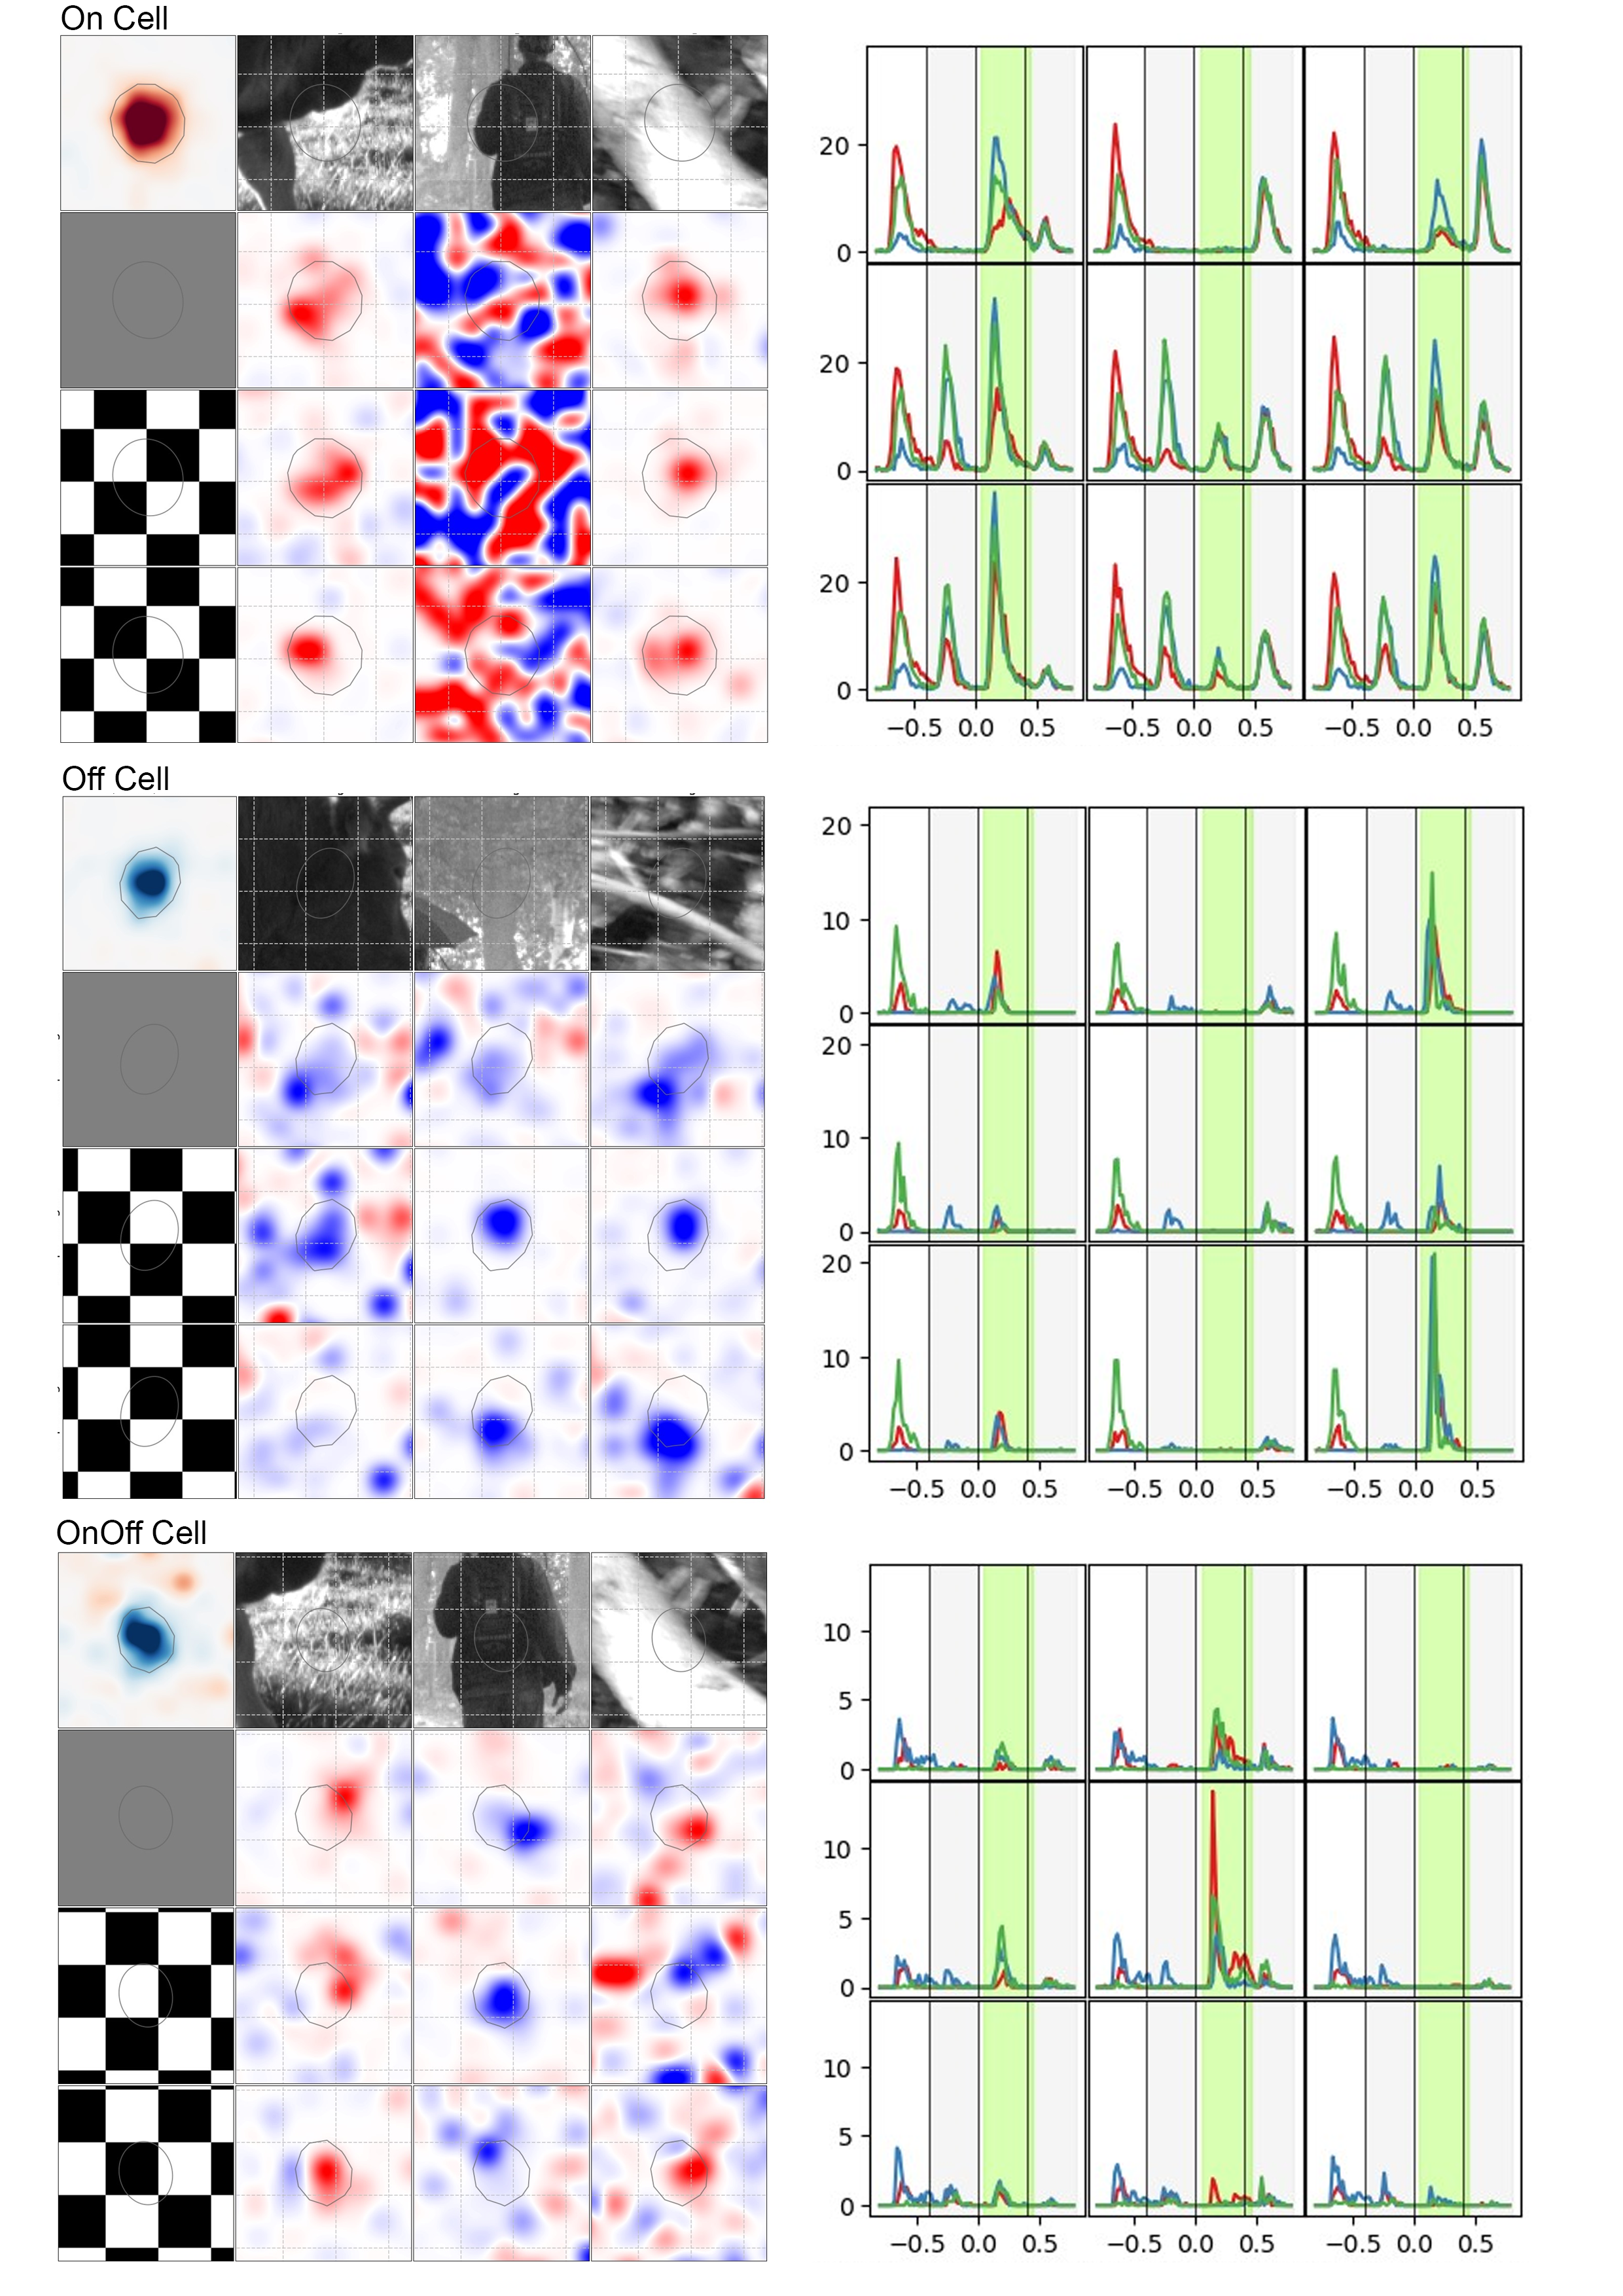
\includegraphics[width=0.8\textwidth]{pics/ExamplePSTHLSTA.png}
    \caption{\textbf{Temporal and spatial aspects of the response depend on
            previous light patterns: some
            exemplary RGCs.} \small	   \textbf{Left} Local Spike Triggered
        Average (LSTA), the average of the
        perturbation checkerboard patterns weighted by the number of spikes
        they
        evoked. Here we centered the view on the RGC receptive field and
        smoothed the
        LSTA using exponential tuning and spatial interpolation. We also
        display the STA in the top-left corner.
        \textbf{Right} Poststimulus time histograms
        (PSTH) are
        histograms of the times at which neurons fire.
        The disposition of the graph follows the same pattern as on the left.
        In each plot, the time
        bins in
        grey corresponds to the display of an adaptation pattern while time
        bins
        in
        white natural images.
        The time axis is centered on the moment when the current natural image
        is displayed. So in order the four rectangles are the previous natural
        image,
        current adaptation pattern, current natural image, and next adaptation
        pattern.
        The area highlighted in yellow corresponds to the 400 ms windows over
        which
        spikes are integrated to compute the LSTA.
        Each color corresponds to a different 'previous natural image'
        displayed 800ms before the current natural image.}
    \label{fig:CellExample}
\end{figure}

\textbf{Can a convolutional neural network model account for this dependence?}
We trained a convolutional neural network (CNN) model to predict the RGC
response to natural images. We hope to infer some of the governing
non-linearities in the recorded RGC. We expect the CNN model to have
good test performance on clips using the gray adaptation since it is trained on
such data However it's unclear how it will generalize to the other two
adaptation patterns. Additional divisive dynamics such as gain control would
have to be added to the model. More on model design can be found in Methods and
Appendix.

Here, we will show the results obtained from one of our models on one single
cell.
First, as we expected, the model predicted the clip using the gray adaptation
better and mostly failed in the other two cases (Figure
\ref{fig:CNNResults}.a). Notice that in most cases it
did predict a response but did not account for the new delay.
This hints at temporal dynamics being not well encoded in the CNN model.

However, test performances are not enough to validate a model that can be used
to build a hypothesis on the retinal code. We also have to make sure that the
model learns its filters to look like those of retinal cells. In the subunit,
we expect a center/surround spatial filter with a biphasic temporal filter. In
the RGC, we expect a localized receptive field, preferentially with a
center/surround spatial filter with a biphasic temporal filter. As shown in
Figure \ref{fig:CNNResults}.b, while the chosen model has a localized RGC
receptive field
with a slightly biphasic temporal filter, it lacks a clear surround in the
filter
of its subunits. As a consequence of the filters being too small, there are
large discontinuities on the border of the subunit filters that are not
desirable.
The structure of the filters is influenced by the L1 and L2 regularization that
are difficult to find tuned.

Finally, we would like to know if the CNN model can predict the displacement of
the LSTA observed before. We computed the LSTA as the average gradient of the
model over the frame of the stimulus that contained the natural image. This computation method is still in development. It seems
that the current model is not able to predict this displacement (Figure
\ref{fig:CNNResults}.c). This could
indicate that it structurally can't learn them, which would go in favor of
extending the model with more complex temporal dynamics such as gain control.
But it could also mean that the model was not properly trained.

\begin{figure}
    \centering
    \vspace*{-3cm}
    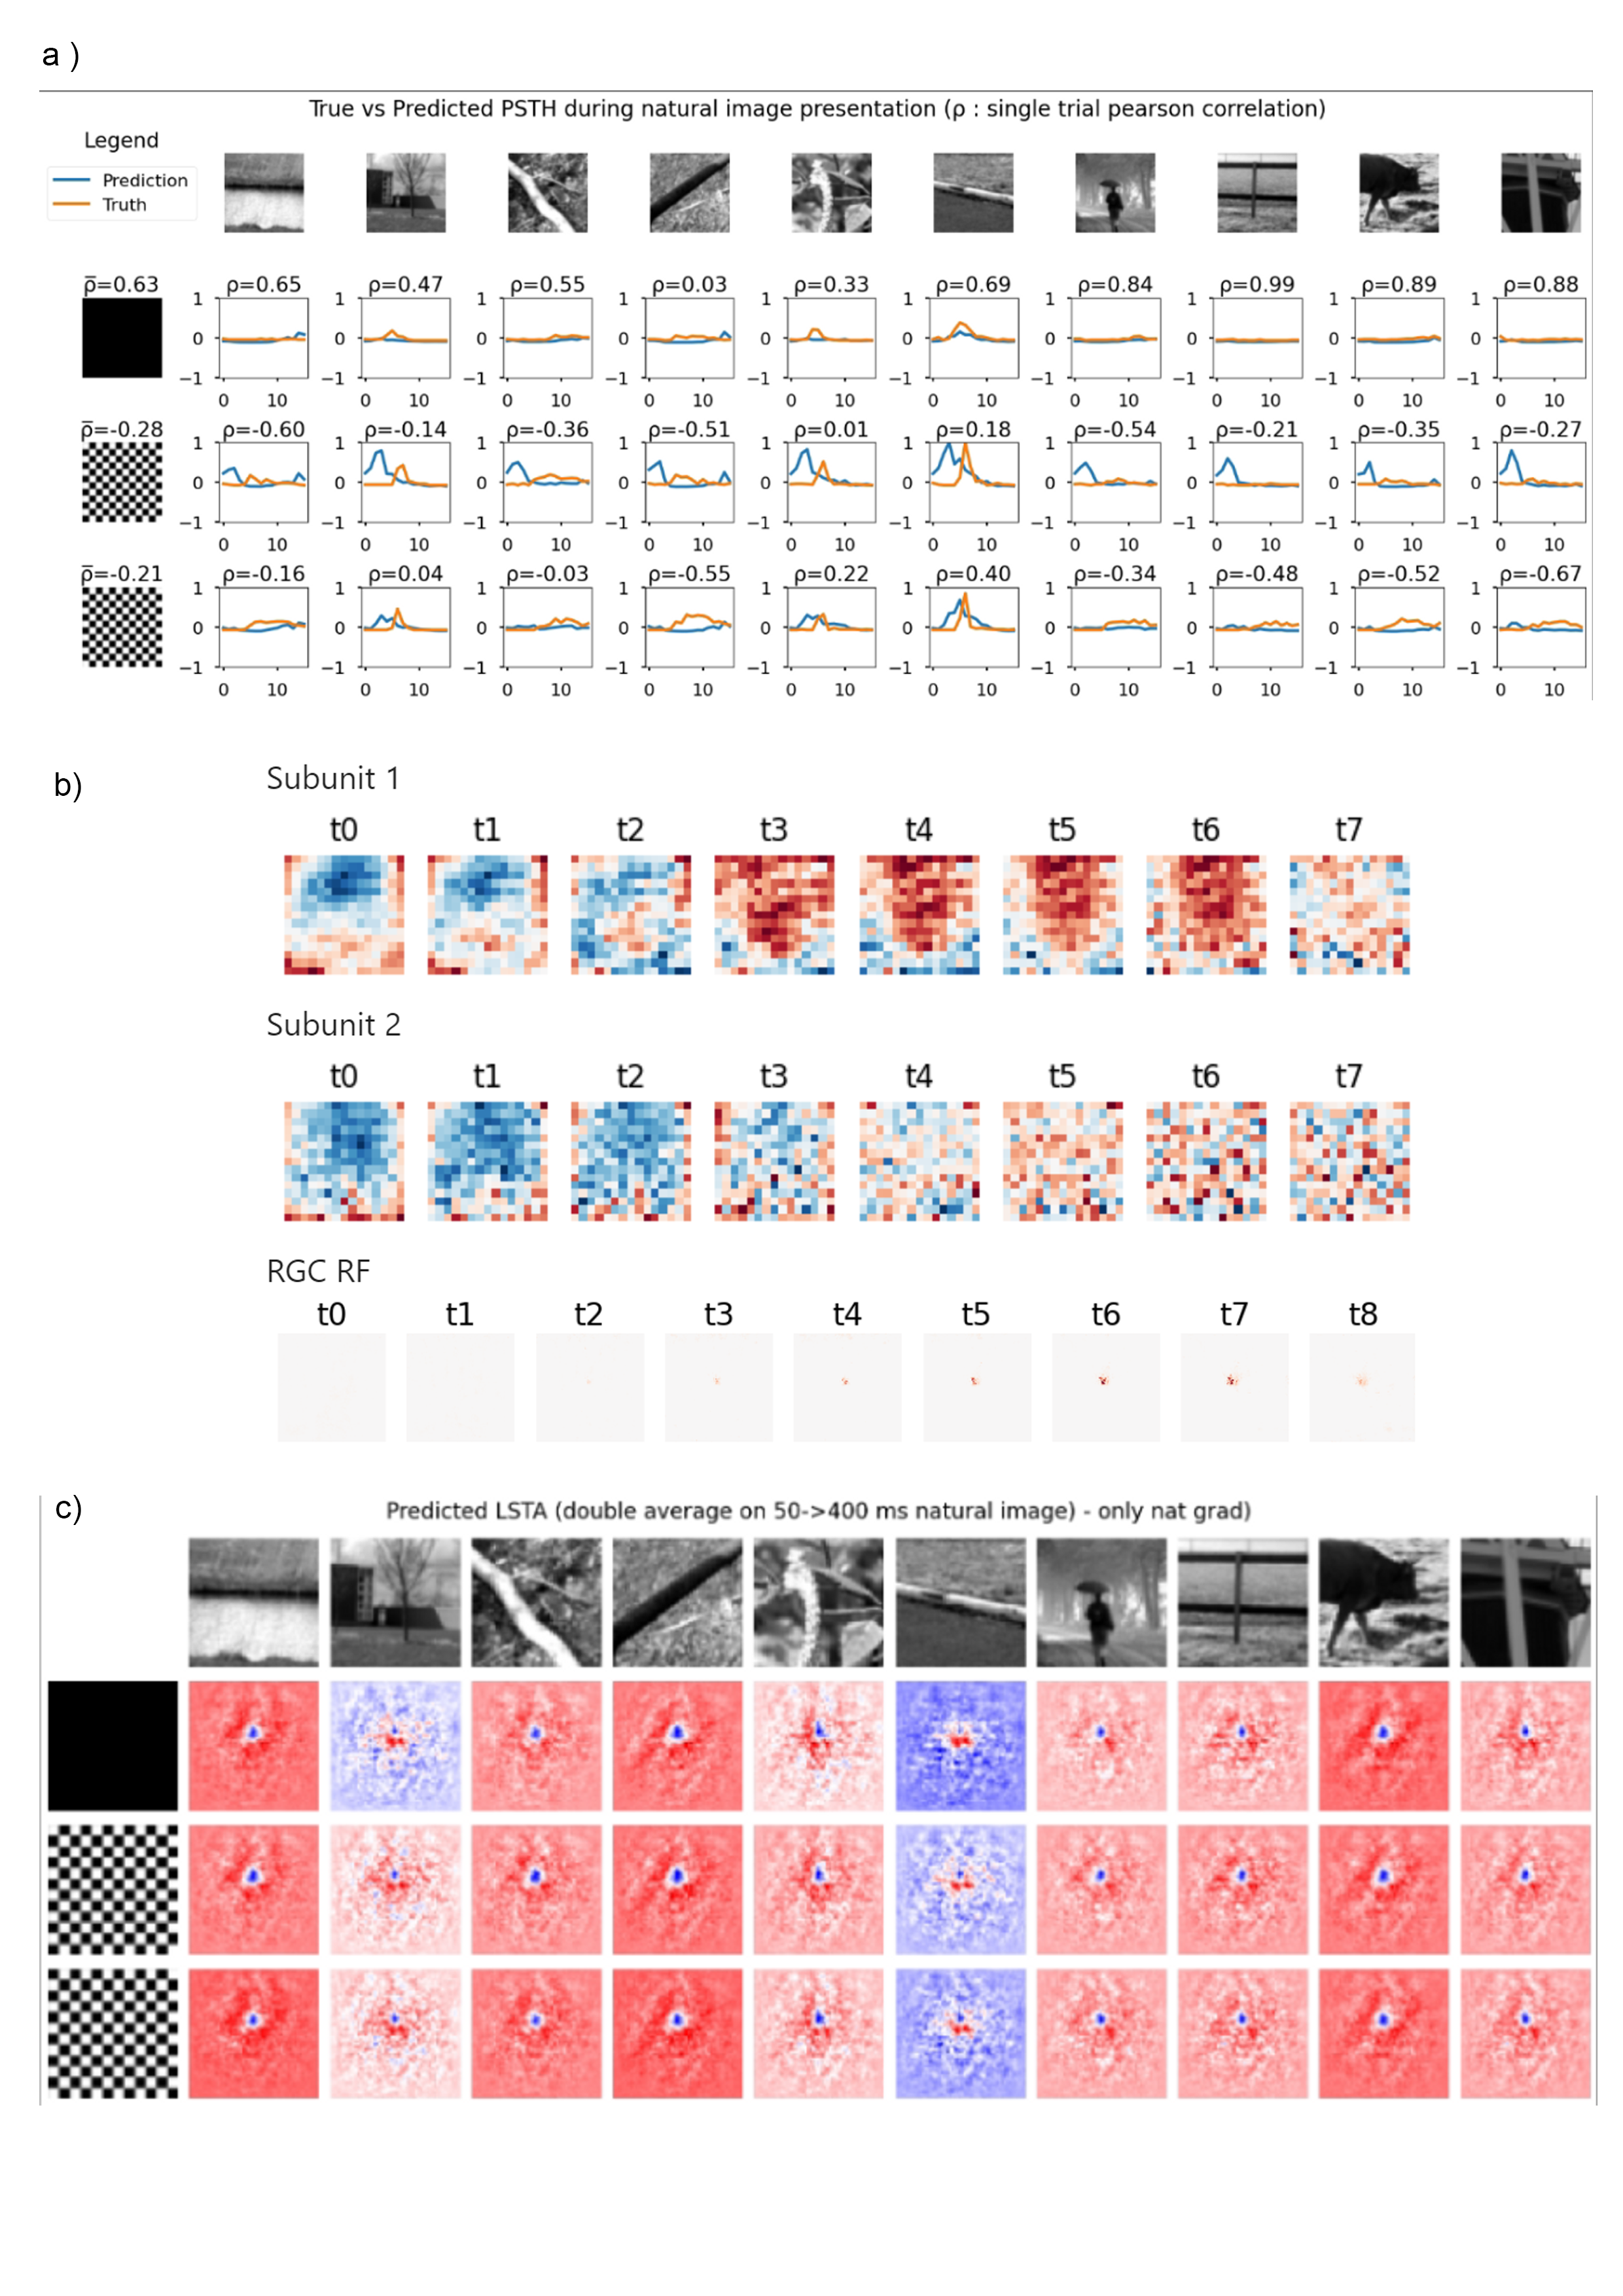
\includegraphics[width=\textwidth]{pics/CNNResults.png}
    \caption{\textbf{Resluts from the CNN model.} \textbf{a.} Single trial
        correlation $\rho$ performance
        of the CNN model on the three different adaptation patterns (see
        Methods). The model
        was
        trained on the gray adaptation pattern. \textbf{b.} Filters of the
        subunits and
        RGCs of the CNN model. \textbf{c.} LSTA computed from the CNN model.}
    \label{fig:CNNResults}
\end{figure}

\clearpage
\section{Methods}\label{sec:methods}

This work is in some ways a continuation of
\cite{goldin_context-dependent_2022}, from which we derived most of the methods
presented here. By comparison, this time we take account of temporal dynamics
in the responses. The switch from 2D visual inputs to 3D spatio-temporal inputs
complexifies every steps of the analysis but is ... COMPLETE

\textbf{Retinal recordings.}
Since I don't realize any experiments myself, I will try here to give as few
details
as necessary for the understanding of the rest of the work. Still, experimental
recording of the retina is a very interesting topic and the reader can look
here for more information. % Useful ?
The laboratory has access to three experimental rooms that enable
state-of-the-art experimentation
on the retina.	For this project, we record the activity of retinal ganglion
cells
using a multi-electrode array. The retina is placed on a ???
% TO COMPLETE

% A part to complete

\textbf{Stimuli design.}
The stimuli used in this project are composed of two images, one synthetic
adaptation image followed by a natural image. Adaptation images are taken from
a pull of three different patterns: a grey screen used as control, a
checkerboard of X*X checks and the same checkerboard with inverted colors (Fig.
TO ADD). Natural images are taken from ADD REFERENCE. XXXX images were used for
training the CNN, 10 were used to test the CNN and among them, 3 were used to
record an estimation of the LSTA of each cell.
Adaptation and natural images are always paired together to form a single
stimulus pair, also referenced as a clip. Each frame is XXXxXXX pixels wide and
each clip is 2*400ms long.

% Give details about how the images are built for the camera?

The training set is composed of XXXX clips, each composed of the grey
adaptation image followed by a natural image. The test set is composed of 30
clips, each repeated 30 times. The test clips are composed of 10 different
natural
images preceded by each adaptation (3 different clips for each natural image).
The dataset used to record LSTA is composed of 9 different clips repeated 1000
times. Each clip is composed of one of the three selected natural images
preceded by one of the adaptation patterns.

We first used 4 different natural images while computing the LSTA of each cell,
each 12 different clips being repeated 12 times. We found that the estimation
of the LSTA was too unstable with only 750 repetitions. In following
experiments we excluded the image that yielded the least amount of stable
estimations of LSTA (20\% average success rate as compared to 42\% average
success rate for the other three images). We then used 3 different natural
images while computing the LSTA of each cell, each 9 different clips being
repeated 1000 times. We found that the estimation of the LSTA was stable with
1000 repetitions.

\textbf{Data processing.}
Multi-electrode array experimental data takes the shape of a collection of
temporal electrical signals tiling the recorded area.
In most scenarios, including here, these signals are sorted into different cell
signals using a semi-automatic algorithm. This algorithm is based on the shape
of the electrical spikes as well as their spatial location. It is
quite messy due to the low signal-to-noise ratio in the data and each
experiment
needs to have its sorting corrected by hand. This process can take up to an
entire day for a single experiment. I used spiking-circus for semi-automatic
spike sorting and the UI phy for handmade corrections. [CITE]
It is important to note that even though the retina is an easier organ than
most to record clean spike signals from, the data is still very noisy and the
sorting process is not perfect. Hence, when validating hypotheses, cells are
usually rated by their reliability.

% Checkeckerboards and RF
After spike sorting, we analyze the recording from standard stimuli to
characterize each
ganglion cell receptive field. To this end, we display a random binary
checkerboard for approximately 1 h at 30 Hz. Check size is 42\microns. A
ganglion cell receptive is computed as its spike trigger average (STA), for
this checkerboard stimulus. The STA of a cell can also be described as the
stimulus that triggers the most spikes from that cell. It is computed as the
average of the presented checkerboard weighted by the number of spikes using a
set number of samples per repetition (here 21). The spatial STA is usually
shown as the 2-dimensional spatial slice at the maximum value after smoothing.
Temporal STA is the one dimensional time slice at the pixel with the maximum
value. For smoothing, a double Gaussian is fitted on the resulting spatial
STA.

% Cell typing (probably useless here, but say a word about it)

% Nat images
\textbf{Natural images.}
We used a subset of the Open Access van Hateren Natural Images Dataset [ADD TO
        BIB]. It consists of monochromatic and calibrated (perfect mapping from
pixel
value to luminance) images of diverse natural environments. These images need
to
be preprocessed to avoid triggering the adaptation to different ranges of light
intensities in the retina, which would call unwanted
dynamics. First, images with numerous saturated pixels were not included in our
subset. Using a custom procedure previously developed in the laboratory, we
then
ensured the images were normalized in the mean luminance and the root mean
square (RMS) contrast.

\textbf{LSTA.}
To record the local specoficity of the response of a ganglion cell to a natural
image, we used a method called local spike trigger average (LSTA) for its
analogy with the STA. This method was previously developed in the laboratory.
We first generate a set of perturbed natural images by superimposing some of
the natural images (3-4 images) with various perturbation patterns in the form
of random checkerboards. We once again used a checker size of 42\microns.
Following calibration guidelines measures in previous experiments, the
amplitude of the perturbation was set to 12.5\%, where 100\% corresponds to a
pixel value of 1. In the mouse retina, this amplitude was found to trigger a
change in firing rate of approximately 1.5Hz in ganglion cells with high firing
rates to the unperturbed images \citep{goldin_context-dependent_2022}.

\textbf{Data visualization.}
Due to the diversity of the data we work with, it can be challenging to have
all the relevant information on one screen. First, it's important to always
have the rasterplot in sight since it informs of the quality of the cell at a
glance. I u

\textbf{Data selection.}
Not all recorded cells are suitable for all types of analysis. Overall, the
main
quality we look for in a cell is its stability during an entire stimulus clip.
It reflects its health and likeliness to behave normally during the
presentation. For our most complex experimentations, cells need to remain
stable in-vitro for up to five hours, which is quite unlikely. In Fig. , we
describe the different selection steps and their influence on the amount of
usable data.
Tp
% Graph idea : All type of rasters for one cell
% Bar chart representing the fading amount of data that can used for modeling

Blablable to share my programming skills to help and improve the data pipeline
of
the
laboratory.

% Models : Put the emphasis on the balance between G.C. and data-driven models
% Also insist on the time component of the models
\textbf{Modeling.} This should be the main part of my internship and also the
most challenging. We are designing a dynamical model of the retinal fast
adaptation. In fact, we mostly look at the evolution of the response from an
image to another, meaning that the dynamic we observe only spans two points in
time. This reduction makes the model more realistic to study. Most of this job
can be summarized as model design, python programming, sensitivity analysis and
data fitting. By comparing how different modeling strategies reproduce the
observed LSTA in the data, we can gain insight on how fast adaptation to
natural scene is implemented in the retina.
%I think what is missing here is what question you want to answer with this. We should discuss this more. 

Our baseline model is the LNLN model of ganglion cell widely used in the
literature. Each neuron is encoded as a spatial linear filter chained with a
non-linearity (usually an activation linearity in the like of ReLU). A single
layer of subunit neurons, representing bipolar cells, converge into a single
modeled ganglion cell.	We would like to add temporal dynamics to this model,
either by adding a time dimension to the spatial liner filter of the cells or
by considering a gain control mechanism. This last mechanism consists in
scaling up or down the present output depending on past outputs (Figure
TO FIND~\cite{}).

\begin{figure}
    \centering
    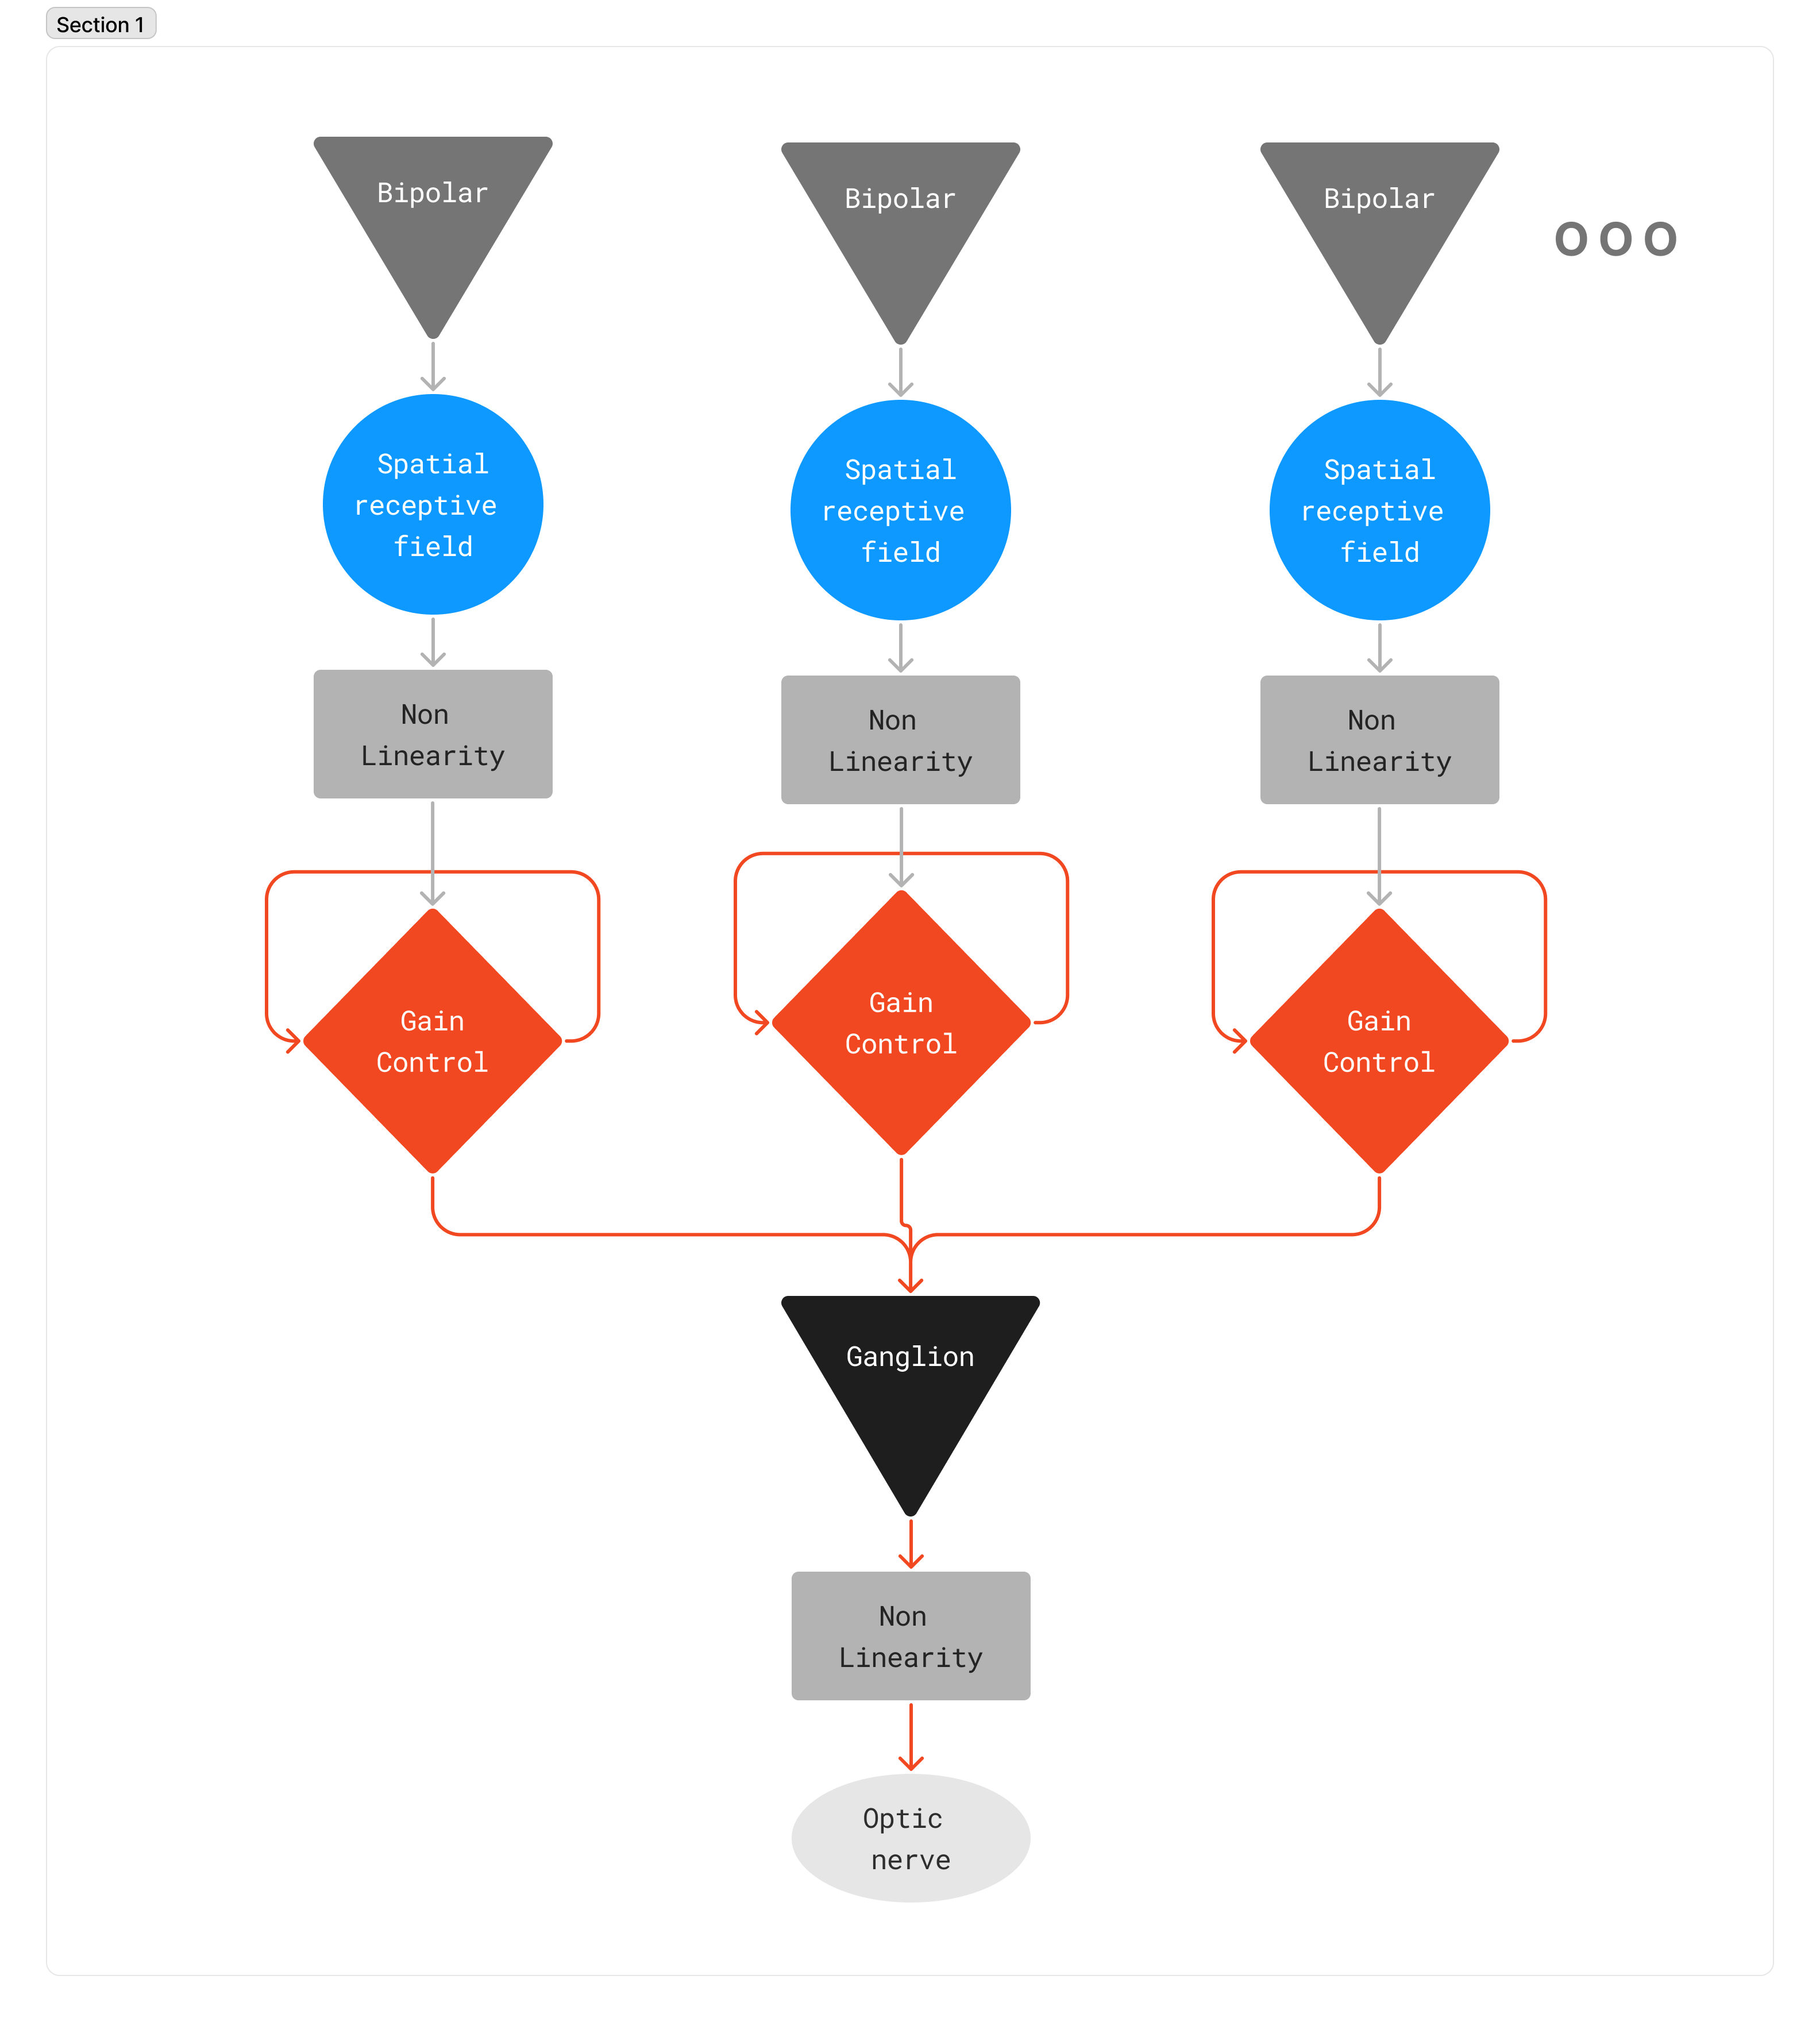
\includegraphics[scale = 0.2]{pics/GCModelDiagram.png}
    \caption{\textbf{Quick sketch of a gain control LNLN model.} Each bipolar
        cell is
        composed of a linear spatial filter that selectively responds to part
        of the scene,
        a non-linear activation function, and a gain control mechanism that
        scale its output
        depending on past events. They all converge into on bipolar cell
        (forming its receptive field)
        of which output is also modeled using a non-linear function.}
    \label{fig:LNLN}
\end{figure}
We will first study our models in a data agnostic manner and study its behavior
for different set of parameters. We will then fit it on our own experimental
data using an efficient optimization framework in python using strategies
developed in the field of machine learning.

% Your references go at the end of the main text, and before the
% figures.  For this document we've used BibTeX, the .bib file
% scibib.bib, and the .bst file Science.bst.  The package scicite.sty
% was included to format the reference numbers according to *Science*
% style.

%BibTeX users: After compilation, comment out the following two lines and paste in
% the generated .bbl file. 

\bibliography{scibib}

\bibliographystyle{Science}





\section*{Acknowledgments}
Include acknowledgments of funding, any patents pending, where raw data for the paper are deposited, etc.

%Here you should list the contents of your Supplementary Materials -- below is an example. 
%You should include a list of Supplementary figures, Tables, and any references that appear only in the SM. 
%Note that the reference numbering continues from the main text to the SM.
% In the example below, Refs. 4-10 were cited only in the SM.     
\section*{Supplementary materials}
Materials and Methods\\
Supplementary Text\\
Figs. S1 to S3\\
Tables S1 to S4\\
References \textit{(4-10)}


\clearpage

\end{document}




















